\noindent
Spadek gradientowy jest to jeden ze sposobów odnalezienia najlepszej regresji. Używa on do tego funkcję kosztu, do której parametry modyfikuje sobie w zależności od kroku ($\alpha$) oraz pochodnej po kierunku. Wzór na spadek gradientowy powtarzamy aż do otrzymania wszystkich pochodnych równych 0 lub określoną ilość iteracji.
\large
$$
\theta_{j} := \theta_{j} - \alpha \frac{\partial}{\partial\theta_{j}} J(\theta_{0}, \theta_{1})
$$
\normalsize
\noindent
\newline
W zależności od ilości $\theta$ będziemy musieli równocześnie aktualizować tyle nowych $\theta$. Wzór jest w pewnym sensie uproszczeniem, tak naprawdę po lewej stronie nie będą stały $\theta_{j}$, a $\theta_{j}temp$, a na samym końcu wszystkie $\theta$ będą uaktualniane. 


	\begin{figure}[H]
    \centering
    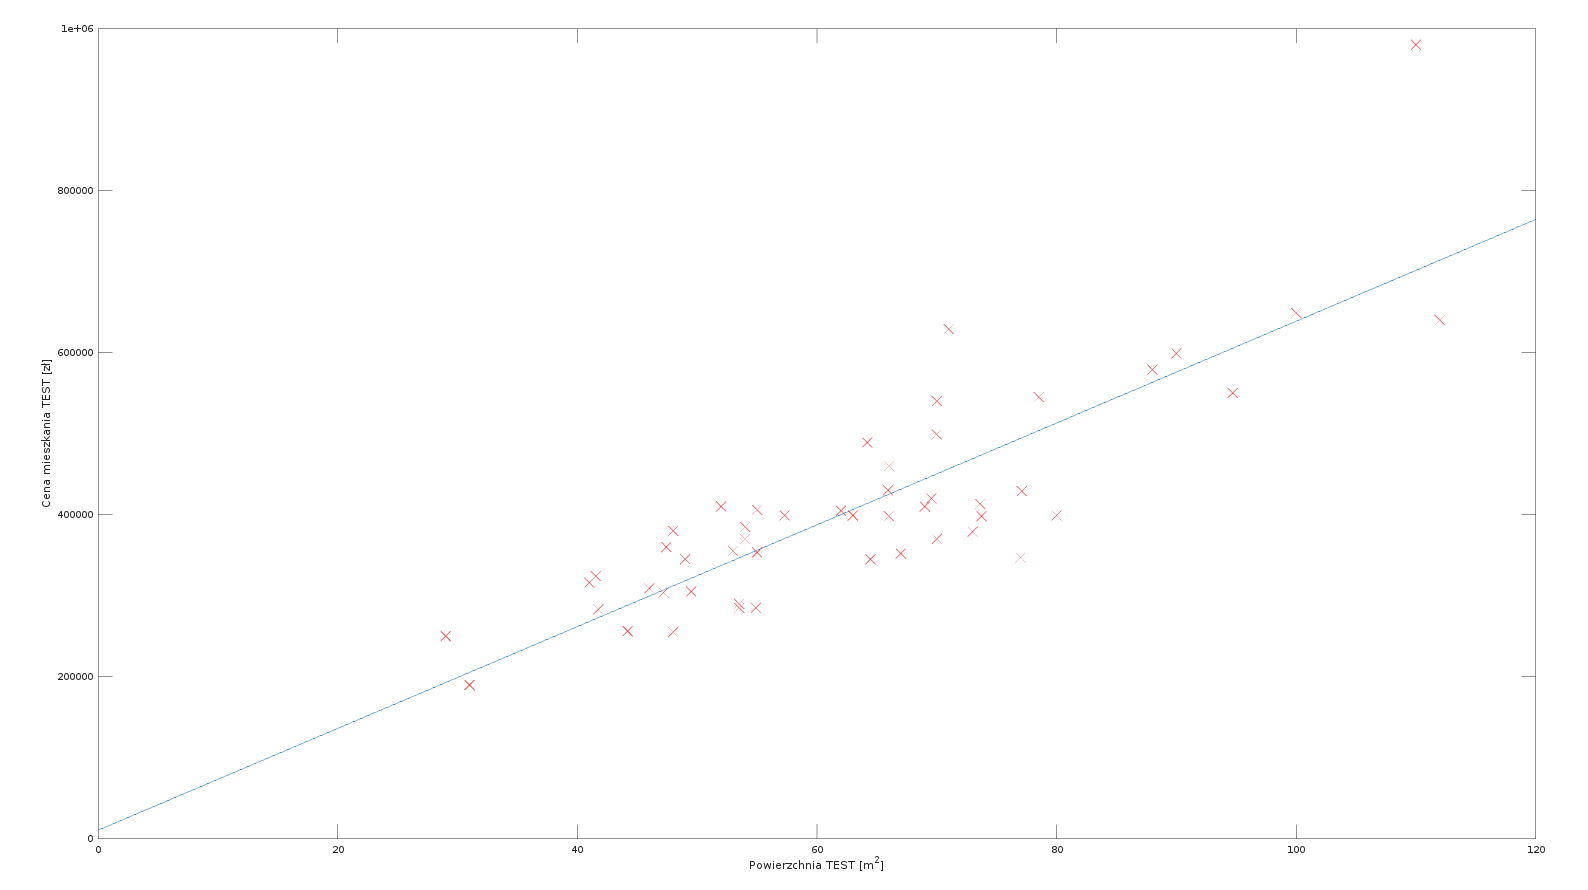
\includegraphics[scale=0.22]{PNG/perfect_grad.png}
    \caption{Idealna regresje znaleziona przez spadek gradientowy}
    \label{lamana}
	\end{figure}
	

- skąd wiemy, że doszliśmy do minimum \\